\documentclass[]{article}
\usepackage{lmodern}
\usepackage{amssymb,amsmath}
\usepackage{ifxetex,ifluatex}
\usepackage{fixltx2e} % provides \textsubscript
\ifnum 0\ifxetex 1\fi\ifluatex 1\fi=0 % if pdftex
  \usepackage[T1]{fontenc}
  \usepackage[utf8]{inputenc}
\else % if luatex or xelatex
  \ifxetex
    \usepackage{mathspec}
  \else
    \usepackage{fontspec}
  \fi
  \defaultfontfeatures{Ligatures=TeX,Scale=MatchLowercase}
\fi
% use upquote if available, for straight quotes in verbatim environments
\IfFileExists{upquote.sty}{\usepackage{upquote}}{}
% use microtype if available
\IfFileExists{microtype.sty}{%
\usepackage{microtype}
\UseMicrotypeSet[protrusion]{basicmath} % disable protrusion for tt fonts
}{}
\usepackage[margin=1in]{geometry}
\usepackage{hyperref}
\hypersetup{unicode=true,
            pdftitle={Guía de trabajos prácticos Bioestadística II: Análisis de poder y primera tarea},
            pdfauthor={Derek Corcoran},
            pdfborder={0 0 0},
            breaklinks=true}
\urlstyle{same}  % don't use monospace font for urls
\usepackage{longtable,booktabs}
\usepackage{graphicx,grffile}
\makeatletter
\def\maxwidth{\ifdim\Gin@nat@width>\linewidth\linewidth\else\Gin@nat@width\fi}
\def\maxheight{\ifdim\Gin@nat@height>\textheight\textheight\else\Gin@nat@height\fi}
\makeatother
% Scale images if necessary, so that they will not overflow the page
% margins by default, and it is still possible to overwrite the defaults
% using explicit options in \includegraphics[width, height, ...]{}
\setkeys{Gin}{width=\maxwidth,height=\maxheight,keepaspectratio}
\IfFileExists{parskip.sty}{%
\usepackage{parskip}
}{% else
\setlength{\parindent}{0pt}
\setlength{\parskip}{6pt plus 2pt minus 1pt}
}
\setlength{\emergencystretch}{3em}  % prevent overfull lines
\providecommand{\tightlist}{%
  \setlength{\itemsep}{0pt}\setlength{\parskip}{0pt}}
\setcounter{secnumdepth}{0}
% Redefines (sub)paragraphs to behave more like sections
\ifx\paragraph\undefined\else
\let\oldparagraph\paragraph
\renewcommand{\paragraph}[1]{\oldparagraph{#1}\mbox{}}
\fi
\ifx\subparagraph\undefined\else
\let\oldsubparagraph\subparagraph
\renewcommand{\subparagraph}[1]{\oldsubparagraph{#1}\mbox{}}
\fi

%%% Use protect on footnotes to avoid problems with footnotes in titles
\let\rmarkdownfootnote\footnote%
\def\footnote{\protect\rmarkdownfootnote}

%%% Change title format to be more compact
\usepackage{titling}

% Create subtitle command for use in maketitle
\newcommand{\subtitle}[1]{
  \posttitle{
    \begin{center}\large#1\end{center}
    }
}

\setlength{\droptitle}{-2em}
  \title{Guía de trabajos prácticos Bioestadística II: Análisis de poder y
primera tarea}
  \pretitle{\vspace{\droptitle}\centering\huge}
  \posttitle{\par}
  \author{Derek Corcoran}
  \preauthor{\centering\large\emph}
  \postauthor{\par}
  \predate{\centering\large\emph}
  \postdate{\par}
  \date{March 14, 2018}

\usepackage{booktabs}
\usepackage{longtable}
\usepackage{array}
\usepackage{multirow}
\usepackage[table]{xcolor}
\usepackage{wrapfig}
\usepackage{float}
\usepackage{colortbl}
\usepackage{pdflscape}
\usepackage{tabu}
\usepackage{threeparttable}
\usepackage[normalem]{ulem}

\begin{document}
\maketitle

{
\setcounter{tocdepth}{2}
\tableofcontents
}
\subsection{Obejtivos del práctico}\label{obejtivos-del-practico}

\begin{itemize}
\tightlist
\item
  Entender cálculos de poder en base a matriz de confusión
\item
  Primera tarea de prácico
\end{itemize}

\subsection{Matriz de confusión}\label{matriz-de-confusion}

La matriz de confusión es una herramienta de toma de desiciones, en el
caso especial de la toma de desiciones tenemos la siguiente matriz de
confusión

\begin{longtable}[]{@{}lll@{}}
\caption{Tabla de confusión de errores}\tabularnewline
\toprule
& Hipótesis nula cierta & Hipótesis alternativa cierta\tabularnewline
\midrule
\endfirsthead
\toprule
& Hipótesis nula cierta & Hipótesis alternativa cierta\tabularnewline
\midrule
\endhead
Acepto hipótesis nula & No hay error & Error tipo 2\tabularnewline
Acepto hipótesis alternativa & Error tipo 1 & No hay
error\tabularnewline
\bottomrule
\end{longtable}

Esto puede ser facilmente ejemplificado con el problema de una alarma de
humo, en este caso cuando la alarma suena y no hay fuego y suena la
alarma tenemos un error de tipo 1, en cambio si hay fuego y la alarma no
suena tenemos un error de tipo 2

\begin{longtable}[]{@{}lll@{}}
\toprule
& No hay fuego & Hay fuego\tabularnewline
\midrule
\endhead
No suena alarma & No hay error & Error tipo 2\tabularnewline
Suena alarma & Error tipo 1 & No hay error\tabularnewline
\bottomrule
\end{longtable}

\subsubsection{Poder y matriz de
confusión}\label{poder-y-matriz-de-confusion}

\begin{itemize}
\tightlist
\item
  Probabilidad de que suene la alarma cuando no hay fuego

  \begin{itemize}
  \tightlist
  \item
    \(\alpha\) usualmente 5\%
  \item
    una de cada 20 alarmas es falsa
  \item
    ¿Cuál es el \(\alpha\) de una alarma de auto?
  \end{itemize}
\item
  Probabilidad de que no suene la alarma cuando hay fuego

  \begin{itemize}
  \tightlist
  \item
    \(\beta\) si es 10\% uno de cada 10 fuegos no es detectado
  \item
    poder es \(1-\beta\) confianza de que fuegos son detectados
  \end{itemize}
\end{itemize}

\subsection{Calculo de poder en R}\label{calculo-de-poder-en-r}

Para hacer calculos de poder en ANOVAS de una y dos vías en \emph{R},
utilizamos el paquete \emph{pwr2}. En este paquete podemos utilizar la
función \emph{pwr.1way} para determinar el poder de un ANOVA de una vía,
los argumentos de esta funcion son:

\begin{itemize}
\tightlist
\item
  \emph{K}: El número de grupos a testear
\item
  \emph{n}: Número de individuos por grupo
\item
  \emph{Alpha}: Nivel de significancia
\item
  \emph{Delta}: Valor mínimo a detectar
\item
  \emph{Sigma}: Desviación estandar de la muestra
\end{itemize}

Para calculos precisos de n necesarios para muestras usar la siguiente
app \url{https://derek-corcoran.shinyapps.io/MinimosCuadrados/}

\subsection{Tarea}\label{tarea}

\subsubsection{El problema}\label{el-problema}

Una compañía que genera pesticidas descarga parte de sus desechos a un
río. La ONG \textbf{RioSano}, dice que ha notado una alza en la
mortalidad de los patos cortacorriente (\emph{Merganneta armata}) del
río.

Ante esto la empresa contrata un científico, el cual hace una estimación
de la mortalidad de patos en 10 zonas del río en que descargan sus
desechos, y lo compara con otros dos ríos no contaminados. Este
científico dice que no hay diferencias significativas en la mortalidad
de los patos de los ríos con desechos y sin desechos con una confianza
del 95\%. Para esto muestra como evidencia la figura 1 y tabla 3 e
incluso hace públicos sus datos en el archivo \emph{MuestraPatos.csv}.

\begin{figure}
\centering
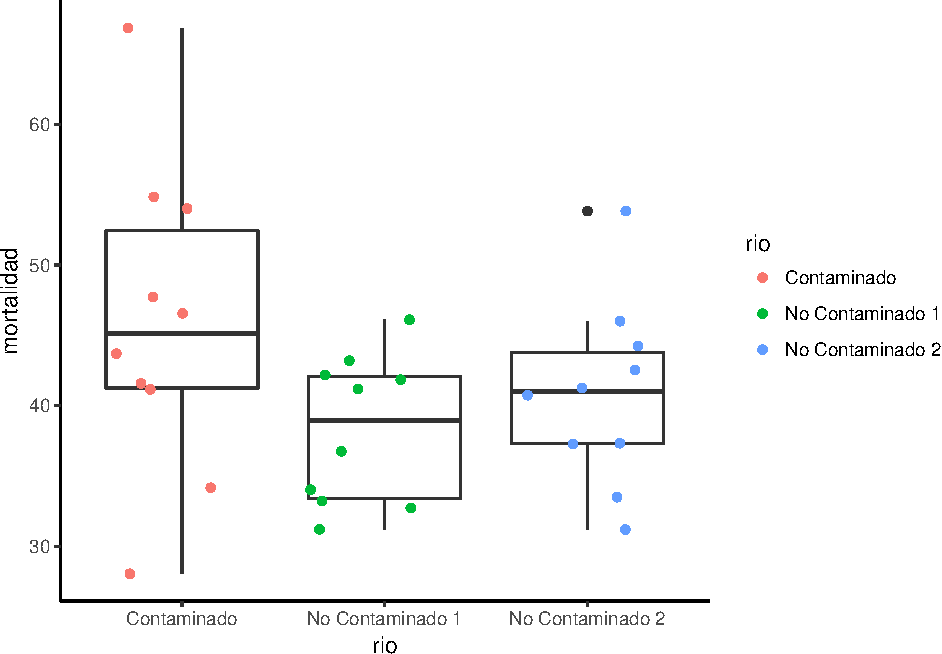
\includegraphics{Guia4_files/figure-latex/unnamed-chunk-3-1.pdf}
\caption{Mortalidades calculadas en 10 zonas de tres ríos}
\end{figure}

\begin{longtable}[]{@{}lrrrrr@{}}
\caption{Tabla de ANOVA de una vía de la mortalidad de patos de los tres
ríos}\tabularnewline
\toprule
term & df & sumsq & meansq & statistic & p.value\tabularnewline
\midrule
\endfirsthead
\toprule
term & df & sumsq & meansq & statistic & p.value\tabularnewline
\midrule
\endhead
rio & 2 & 301.2531 & 150.62656 & 2.359899 & 0.1136188\tabularnewline
Residuals & 27 & 1723.3436 & 63.82754 & NA & NA\tabularnewline
\bottomrule
\end{longtable}

La ONG \emph{RioSano} lo contrata para determinar la validez del estudio
y si es necesario generar un estudio extra. Ante esto:

\begin{enumerate}
\def\labelenumi{\arabic{enumi}.}
\item
  Genere una matriz de confusión del problema y explique en este
  contexto que significaría el alfa y beta para este problema, y cual
  consideraría más relevante.
\item
  Diseñe el estudio que le gustaría hacer, determinando cuantas áreas
  debe muestrear por río, estime un delta mínimo que le gustaría
  determinar y el beta con el que se siente seguro y determine el
  \emph{n} mínimo necesario para ese estudio. Justifique su respuesta
\item
  Dado este \emph{n} mínimo realice lo siguiente

  \begin{itemize}
  \tightlist
  \item
    Realice un muestreo de n muestras por tipo de río del archivo
    \emph{Patos.csv}
  \item
    Genere gráficos y tablas exploratorias de los datos de su muestreo y
    describalas
  \item
    Revise los supuestos del ANOVA para su base de datos tanto
    gráficamente como con tests y determine si se puede realizar el
    anova
  \item
    Diga si según su diseño hay diferencias significativas en la
    mortalidad de patos entre los ríos
  \end{itemize}
\item
  Cada zona a muestrear requiere de un monitoreo exahustivo, que tiene
  un costo de 500.000 pesos (esto es 1.500.000 de pesos si consideramos
  los 3 ríos). La ONG \emph{RioSano} consiguió 20.000.000 de pesos para
  este estudio. Dadas esas limitaciones, genere un balance de
  \(\alpha\), \(\beta\) y \(n\) dada esa limitación para hacer el mejor
  estudio posible dadas las consecuencias, justifique su respuesta.
\end{enumerate}

Genere un informe para la ONG \emph{RioSano} incorporando estos 5 puntos
e incluya una introducción, metodología, resultados,
discusión-conclusión y bibliografía, envíe el script de como generó los
resultados


\end{document}
